% Standalone TikZ: generative process + TWO-BRANCH inference pipeline (fig:pipeline)
% Branch A: hand-crafted summaries (PS + PDF l-moments) -> MLP+VMIM compressor
% Branch B: raw noised cubes -> 3D CNN+VMIM compressor
% Compile:  pdflatex pipeline_dag.tex  ->  pipeline_dag.pdf
\documentclass[tikz,border=6pt]{standalone}
\usepackage{amssymb}
\usetikzlibrary{positioning,arrows.meta,fit,backgrounds,calc}
\begin{document}
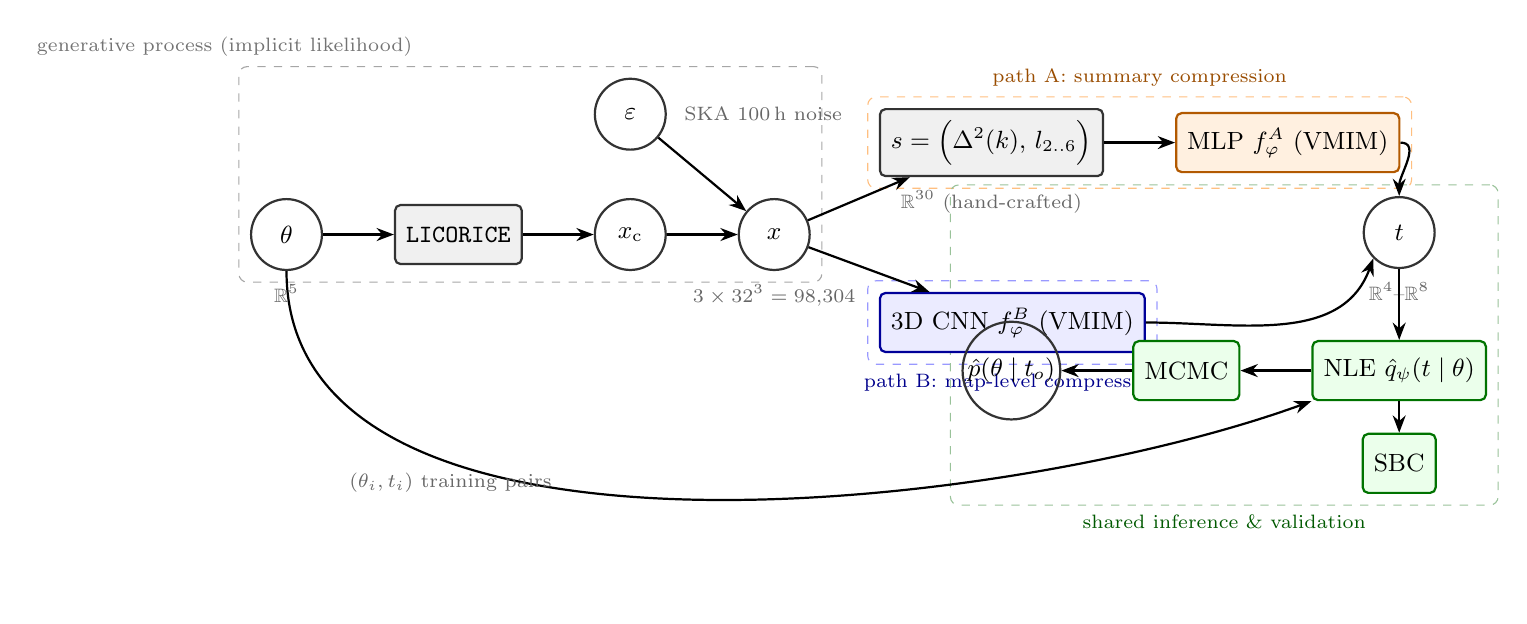
\begin{tikzpicture}[
  font=\small,
  node distance=8mm and 9mm,
  var/.style   ={circle, draw=black!80, thick, minimum size=9mm, inner sep=1pt},
  proc/.style  ={rectangle, rounded corners=2pt, draw=black!80, thick,
                 fill=black!6, minimum height=7.5mm, inner sep=4pt},
  learnA/.style={rectangle, rounded corners=2pt, draw=orange!70!black, thick,
                 fill=orange!12, minimum height=7.5mm, inner sep=4pt},
  learnB/.style={rectangle, rounded corners=2pt, draw=blue!60!black, thick,
                 fill=blue!8, minimum height=7.5mm, inner sep=4pt},
  shared/.style={rectangle, rounded corners=2pt, draw=green!45!black, thick,
                 fill=green!8, minimum height=7.5mm, inner sep=4pt},
  dim/.style   ={font=\scriptsize, text=black!60},
  arr/.style   ={-{Stealth[length=2.2mm]}, thick},
]

% ---------------- generative process ----------------
\node[var] (theta) {$\theta$};
\node[dim, below=0.5mm of theta] {$\mathbb{R}^{5}$};
\node[proc, right=of theta] (sim) {\texttt{LICORICE}};
\node[var, right=of sim] (xc) {$x_{\rm c}$};
\node[var, above=6mm of xc] (eps) {$\varepsilon$};
\node[dim, right=1mm of eps] {SKA 100\,h noise};
\node[var, right=of xc] (x) {$x$};
\node[dim, below=0.5mm of x] {$3\times32^3=98{,}304$};

\draw[arr] (theta) -- (sim);
\draw[arr] (sim) -- (xc);
\draw[arr] (xc) -- (x);
\draw[arr] (eps) -- (x);

% ---------------- branch A: hand-crafted summaries ----------------
\node[proc, above right=4mm and 10mm of x] (hc)
  {$s=\bigl(\Delta^2(k),\, l_{2..6}\bigr)$};
\node[dim, below=0.5mm of hc] {$\mathbb{R}^{30}$ (hand-crafted)};
\node[learnA, right=of hc] (mlp) {MLP $f^{A}_{\varphi}$ (VMIM)};

% ---------------- branch B: raw cubes ----------------
\node[learnB, below right=4mm and 10mm of x] (cnn)
  {3D CNN $f^{B}_{\varphi}$ (VMIM)};

% ---------------- shared tail ----------------
\node[var] (t) at ($(mlp.east)!0.5!(cnn.east) + (16mm,0)$) {$t$};
\node[dim, below=0.5mm of t] {$\mathbb{R}^{4}$--$\mathbb{R}^{8}$};
\node[shared, below=9mm of t] (nle) {NLE $\hat q_\psi(t\mid\theta)$};
\node[shared, left=of nle] (mcmc) {MCMC};
\node[var, left=of mcmc] (post) {$\hat p(\theta\mid t_o)$};
\node[shared, below=4mm of nle] (sbc) {SBC};

\draw[arr] (x) -- (hc);
\draw[arr] (hc) -- (mlp);
\draw[arr] (mlp.east) to[out=0, in=90] (t.north);
\draw[arr] (x) -- (cnn);
\draw[arr] (cnn.east) to[out=0, in=-110] (t.south west);
\draw[arr] (t) -- (nle);
\draw[arr] (theta.south) to[out=-90, in=-160, looseness=0.8]
  node[dim, pos=0.3, below] {$(\theta_i, t_i)$ training pairs} (nle.south west);
\draw[arr] (nle) -- (mcmc);
\draw[arr] (mcmc) -- (post);
\draw[arr] (nle) -- (sbc);

% ---------------- group boxes ----------------
\begin{scope}[on background layer]
  \node[fit=(theta)(sim)(eps)(x), draw=black!35, dashed, rounded corners=3pt,
        inner sep=4pt, label={[black!55]above left:{\scriptsize generative process
        (implicit likelihood)}}] {};
  \node[fit=(hc)(mlp), draw=orange!50, dashed, rounded corners=3pt,
        inner sep=4pt, label={[orange!60!black]above:{\scriptsize path A:
        summary compression}}] {};
  \node[fit=(cnn), draw=blue!40, dashed, rounded corners=3pt,
        inner sep=4pt, label={[blue!55!black]below:{\scriptsize path B:
        map-level compression}}] {};
  \node[fit=(t)(nle)(mcmc)(post)(sbc), draw=green!40!black!40, dashed,
        rounded corners=3pt, inner sep=4pt,
        label={[green!35!black]below:{\scriptsize shared inference \&
        validation}}] {};
\end{scope}

\end{tikzpicture}
\end{document}
